\begin{center}
 \textsc{Физбой, 11 класс. Финал.}
\end{center}
\vspace{0.01cm}
\hrule
\parindent=0mm

\taskpic{Определите сопротивление полубесконечной цепочки между точками
  $A$ и $B$, если сопротивление каждого звена равно $R$.}{
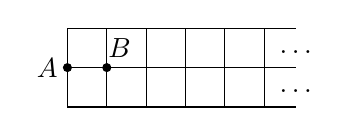
\begin{tikzpicture}
  \draw[step=0.5] (0,0) grid (2.9,1);
  \draw[fill=black] (0,0.5) circle (0.05) node[left] {$A$};
  \draw[fill=black] (0.5,0.5) circle (0.05) node[above=7,right=-3]
  {$B$};
  \draw (2.9,0.2) node {$\ldots$};
  \draw (2.9,0.7) node {$\ldots$};
\end{tikzpicture}
}

\taskpic{Человек, стоя на краю высокого обрыва, смотрит на ровное
  плоское дно котлована шириной $L$, заполненного водой глубины
  $h$. Высота обрыва $H$. Размеры котлована удовлетворяют неравенствам
  $L \gg H \gg h$. Показатель преломления воды равен $n$. Как зависит
  от расстояния до обрыва видимая глубина котлована?}{
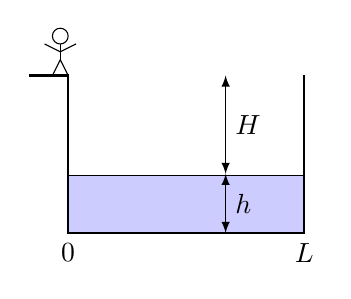
\begin{tikzpicture}[>=latex]
  \draw[fill=blue!20] (1,1) rectangle ++(3,0.73);
  \draw[thick] (0.5,3) -- ++(0.5,0) -- ++(0,-2) -- ++(3,0) --++(0,2);
  \draw[<->] (3,1) -- (3,1.75) node [midway,right] {$h$};
  \draw[<->] (3,1.75) -- (3,3) node [midway,right] {$H$};
  \draw (1,3) -- ++(-0.1,0.2) -- ++(-0.1,-0.2);
  \draw (0.9,3.2) -- ++(0,0.2);
  \draw (0.9,3.3) -- ++(0.2,0.1);
  \draw (0.9,3.3) -- ++(-0.2,0.1);
  \draw (0.9,3.5) circle (0.1);
  \draw (1,0.75) node {$0$};
  \draw (4,0.75) node {$L$};
\end{tikzpicture}
}

\task{ По диаметру астероида, имеющего форму шара, проходит узкий
  тоннель. С поверхности астероида в тоннель бросили камень, сообщив
  ему скорость, равную первой космической для этого астероида. Через
  какое время камень вернётся назад? Известно, что минимальный период
  обращения космических объектов вокруг астероида равен
  $T_0$. Астероид состоит из однородного вещества, а влияние
  гравитационного поля других небесных тел мало. \\
  \textit{Примечание.} Площадь эллипса $S=\pi ab$, где $a,b$ --- длины
  полуосей эллипса.  }

\task{
  На расстоянии $H$ от бесконечной проводящей плоскости находится
  точечный заряд $q_0$. Найти, на каком расстоянии от проекции заряда
  на плоскость в эту плоскость войдёт силовая линия, вышедшая из
  заряда параллельно плоскости. 
}

\task{
  Один конец тонкой гибкой верёвки с линейной плотностью $\rho$ тянут
  с постоянной горизонтальной скоростью на высоте $H$ над шероховатой
  поверхностью. Второй конец верёвки свободен. Длина части верёвки,
  соприкасающейся с поверхностью, равна $l_1$. Найдите длину верёвки
  $l_2$, не касающейся поверхности. Коэффициент трения скольжения
  верёвки по поверхности равен $k$. 
}

\task{
  Предположим, что создан материал с необычной зависимостью
  коэффициента теплопроводности $k$ от температуры. Пластину из такого
  материала поместили между двумя стенками вплотную к ним. Температуры
  стенок поддерживаются постоянными: $T_1 = 160 K$ и $T_2 = 500 K$
  соответственно. Какой тепловой поток установится между стенками,
  если толщина пластины $d=1 \mbox{ см}$, а её площадь $S= 100 \mbox{
    см}^2$? Найдите температуру в среднем продольном сечении пластины
  ($x=d/2$). \\
\textit{Указание.} Тепловой поток $P$ сквозь тонкий слой вещества,
площадь которого равна $S$, а толщина $dx$, равный количеству теплоты,
проходящему через этот слой в единицу времени, прямо пропорционален
разности значений температуры его поверхностей $dT$ и обратно
пропорционален его толщине: $P = - k S \dfrac{dT}{dx}$, где $k$ ---
коэффициент теплопроводности вещества. 
}

\begin{figure}[h]
  \centering
  \begin{tikzpicture}[>=latex,scale=1.2]
    \draw[help lines,xstep=0.6,ystep=0.35] (0,0) grid (3.4,3.5);
    \draw[thick,->] (0,0) -- (3.6,0) node[above=5,left=-5] {\tiny{$T$, K}};
    \draw[thick,->] (0,0) -- (0,4) node[right=23,below] {\tiny{$k$,Вт/(м$\cdot$К)}};
    \coordinate (a) at (0.8,3);
    \coordinate (b) at (3.2,2.3);
    \coordinate (c) at (1.5,4.3);
    \coordinate (d) at (2.2,0);
    \draw[very thick,red] (a) .. controls (c) and (d) .. (b);
    \draw[blue,dashed] (0.92,0.35*9) -- ++(0,-0.35*9);
    \draw[blue,dashed] (0.6*5,0.35*5.5) -- ++(0,-0.35*5.5) node [below=-1] {\tiny{$T_2$}};
    \draw[blue,->] (0.5,-0.2) node[left=-3] {\tiny{$T_1$}} to
    [out=0,in=215] (0.9,-0.05);
    \draw[thick] (0.6*2,0.15/2) -- ++(0,-0.15) node[below] {\tiny{$200$}};
    \draw[thick] (0.6*4,0.15/2) -- ++(0,-0.15) node[below]
    {\tiny{$400$}};
    \draw[thick] (0.1,0.35*5) -- ++(-0.2,0) node[left=-3] {\tiny{$1$}}; 
    \draw[thick] (0.1,0.35*10) -- ++(-0.2,0) node[left=-3] {\tiny{$2$}};  
  \end{tikzpicture}
\end{figure}

% \begin{center}
%   \includegraphics[width=6cm]{fb11_6.png}
% \end{center}\setcounter{notask}{1}
